\documentclass[tikz,border=8pt]{standalone}

\usepackage[T1]{fontenc}
\usepackage{lmodern}
\usetikzlibrary{arrows.meta}

\begin{document}
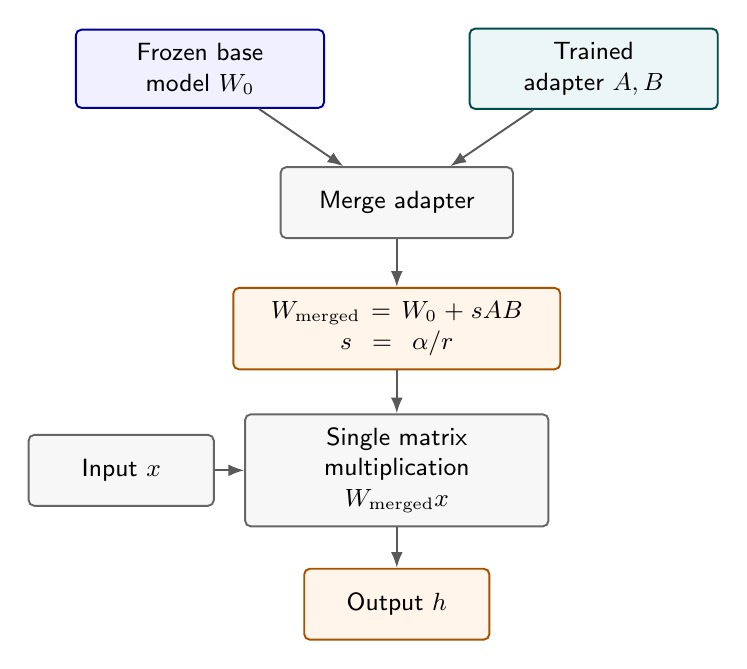
\begin{tikzpicture}[
  font=\sffamily\small,
  block/.style={
    draw=black!60,
    fill=black!3,
    rounded corners=2pt,
    line width=0.7pt,
    minimum height=9mm,
    text width=2.8cm,
    align=center,
    inner sep=5pt,
  },
  frozen/.style={block, draw=blue!60!black, fill=blue!6},
  adapter/.style={block, draw=teal!60!black, fill=teal!7},
  result/.style={block, draw=orange!65!black, fill=orange!8},
  arrow/.style={draw=black!65, line width=0.7pt, -{Latex[length=2mm]}},
]

% Merge the trained low-rank matrices into the pretrained weights.
\node[frozen] (base) at (-2.5,0) {Frozen base model \(W_0\)};
\node[adapter] (adapter) at (2.5,0) {Trained adapter \(A,B\)};
\node[block, text width=2.6cm] (merge) at (0,-1.7) {Merge adapter};
\node[result, text width=3.8cm] (weights) at (0,-3.3)
  {\(W_{\mathrm{merged}}=W_0+sAB\)\\\(s=\alpha/r\)};

\draw[arrow] (base) -- (merge);
\draw[arrow] (adapter) -- (merge);
\draw[arrow] (merge) -- (weights);

% Inference uses the merged matrix in a single multiplication.
\node[block, text width=2.0cm] (input) at (-3.5,-5.1) {Input \(x\)};
\node[block, text width=3.5cm] (multiply) at (0,-5.1)
  {Single matrix multiplication\\\(W_{\mathrm{merged}}x\)};
\node[result, text width=2.0cm] (output) at (0,-6.8) {Output \(h\)};

\draw[arrow] (input) -- (multiply);
\draw[arrow] (weights) -- (multiply);
\draw[arrow] (multiply) -- (output);
\end{tikzpicture}
\end{document}
